\documentclass{article}%
\usepackage[T1]{fontenc}%
\usepackage[utf8]{inputenc}%
\usepackage{lmodern}%
\usepackage{textcomp}%
\usepackage{lastpage}%
\usepackage[head=40pt,margin=0.5in,bottom=0.6in]{geometry}%
\usepackage{graphicx}%
%
\title{\textbf{95\% de los hospitales carece de equipos para hacer diagnósticos}}%
\author{Olgalinda Pimentel R.}%
\date{30/11/2018}%
%
\begin{document}%
\normalsize%
\maketitle%
\textbf{URL: }%
http://www.el{-}nacional.com/noticias/sociedad/los{-}hospitales{-}carece{-}equipos{-}para{-}hacer{-}diagnosticos\_261602\newline%
%
\textbf{Periodico: }%
EN, %
ID: %
261602, %
Seccion: %
Sociedad\newline%
%
\textbf{Palabras Claves: }%
Sociedad\newline%
%
\textbf{Derecho: }%
2.1%
, Otros Derechos: %
2.1%
, Sub Derechos: %
2.1.1, 2.1.1.1%
\newline%
%
\textbf{EP: }%
NO\newline%
\newline%
%
\textbf{\textit{70\% de las 40 instituciones evaluadas en 24 entidades del país, reportó falta de agua y electricidad en una semana, señaló la Encuesta Nacional de Hospitales}}%
\newline%
\newline%
%
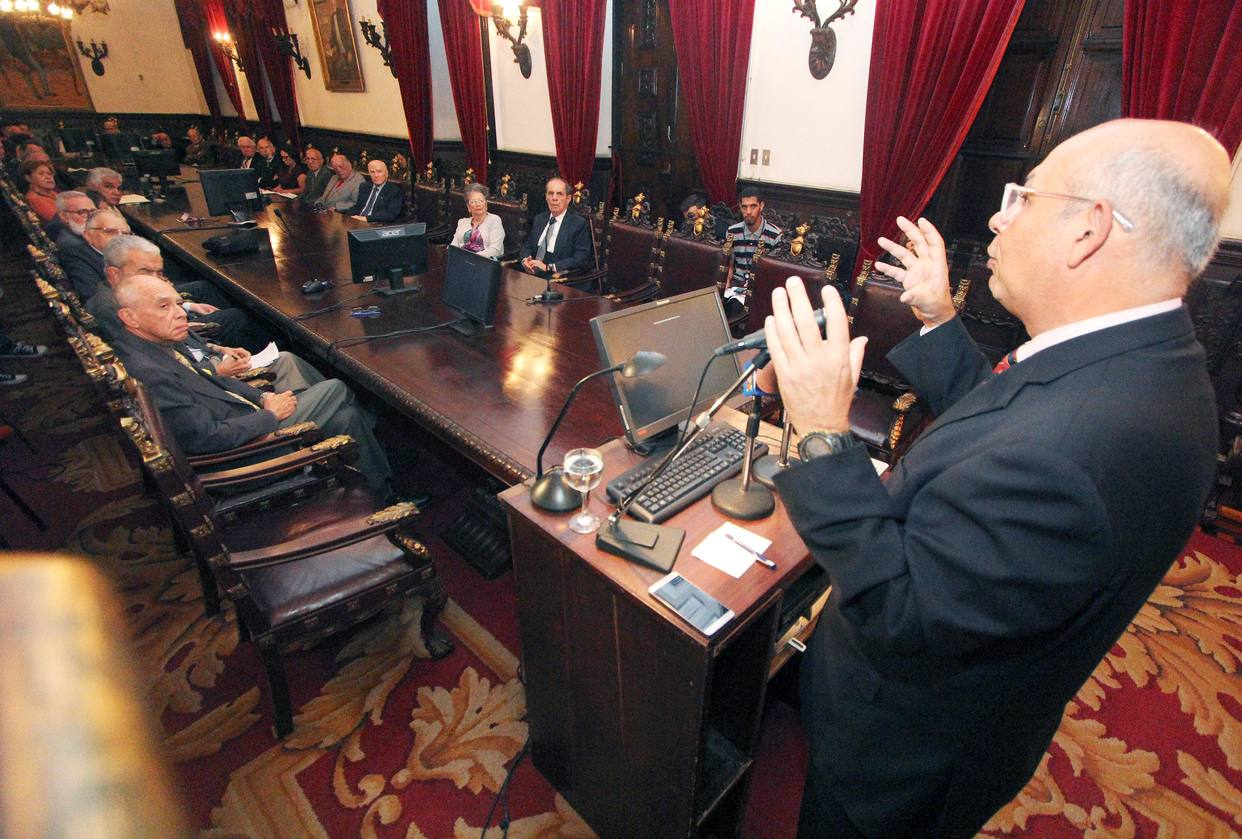
\includegraphics[width=300px]{131.jpg}%
\newline%
%
Hospitales abiertos pero con unidades cerradas o que funcionan de modo intermitente, con severos problemas de servicios como agua y electricidad, con menos camas y escasos medicamentos para atender emergencias, y con médicos y enfermeras insuficientes, es el resultado desalentador de un estudio, el segundo de 2018, realizado por la organización Médicos por la Salud, entre el 10 y el 16 de noviembre, en 40 centros de atención pública (adscritos al ministerio, IVSS, Sanidad Militar y gobernaciones) ubicados en 24 entidades del país. “La salud está comprometida~y la tendencia es a que empeore sistemáticamente”, afirmó el médico infectólogo Julio Castro Méndez, integrante de la ONG, quien expuso el contenido de la Encuesta Nacional de Hospitales, en su segundo reporte, ante los miembros de la Academia Nacional de Medicina y medios.%
\newline%
%
Los académicos expresaron su reconocimiento al trabajo realizado por el equipo de profesionales y mostraron alarma ante la data revelada. “La emergencia no espera en ningún hospital, ¿qué podría hacerse donde ocurra eso?”, preguntó el traumatólogo Claudio Aoün Soulie, individuo de número.%
\newline%
%
33\% de las camas de emergencia se encuentra inoperativa, lo cual anula la posibilidad de atender pacientes en cualquier grado de patología y disminuye, además, el grado de preparación de los médicos, comentó Daniei Golindano, coordinador de la ONG, a quien correspondió la presentación a los medios. Los hospitales más afectados están ubicados en Aragua, Monagas, Falcón y Táchira.%
\newline%
%
La encuesta también señala que se agrava el estado de los servicios de apoyo diagnóstico, lo cual es indicador de la profundización de la crisis hospitalaria: 95\% de los centros de salud examinados no realiza tomografías ni resonancias porque los equipos están dañados; 43,24\%, es decir casi la mitad de la muestra, no tiene capacidad para realizar estudios de laboratorio de ningún tipo porque estos centros se encuentran cerrados; más de la mitad reporta que el servicio de rayos X no funciona y 42,42\% no posee equipos para hacer ecos.%
\newline%
%
Uno de los elementos novedosos de esta segunda entrega es la inclusión de los servicios públicos como indicadores de evaluación. Y es también uno de los más decisivos para determinar la salud de los hospitales. 67,57\% de los centros aseguró que hubo fallas eléctricas en una semana, y de esta cantidad 42\% reportó tener plantas de electricidad en buenas condiciones; del total, en 32,43\% fallaron monitores, incubadoras, ventiladores y desfibriladores, entre otros, durante el apagón.%
\newline%
%
“Se ha ido la luz durante 105,2 horas semanales en todos los hospitales”, puntualiza la encuesta.%
\newline%
%
El problema de agua es similar en los centros asistenciales. En 70\% de estos faltó el suministro regular, y 8\% de los ubicados en Amazonas, Cojedes y en el Distrito Capital (Hospital Vargas) no tuvo el servicio ningún día de la semana.%
\newline%
%
Desabastecidos%
\newline%
%
La encuesta empleó nueva metodología para medir la existencia de medicamentos, a través de dos~score. El primero referido a la emergencia con 20 fármacos imprescindibles, reveló que en 52\% de los centros hospitalarios no hay medicinas necesarias disponibles. El segundo referido a pabellón con 12 ítems, indicó que en 38\% no se cuenta con los implementos básicos ni para operar de apendicitis.%
\newline%
%
“Si nos toca poner medicamentos para la gente, los pondremos”%
\newline%
%
La crisis que no debía afectar a los hospitales por ser estos los receptores de las emergencias de salud, los está perjudicando de manera importante. “Que no haya luz durante 105 horas en una semana es terrible, pero refleja lo que ocurre en el país”, aseveró Julio Castro, quien no descartó que en el tercer estudio sobre el recurso humano, que ya adelantan, la situación sea más compleja en los centros asistenciales.%
\newline%
%
Como representante de Médicos por la Salud envió~un mensaje a los pacientes que no tienen otra opción que recurrir a los hospitales. “Nuestros médicos venezolanos están allí para atenderlos y estar con ellos. La labor de siempre es acompañar en el dolor y si nos toca poner medicamentos, pondremos medicamentos. Un valor fundamental es el compromiso del especialista de estar allí, pase lo que pase, a pesar de la violencia que enfrentan en los centros asistenciales”.%
\newline%
%
Afirmó que a pesar de que el derecho a la salud está en juego, no es optimista sobre una respuesta positiva del gobierno para resolver la emergencia. “Es difícil interpretar el silencio, pero pensamos que nuestra responsabilidad como médicos es hacer este trabajo. Tenemos el pulso en el sistema de salud venezolano y allí estaremos para generar~ información creíble y auditable de lo que ocurre en los hospitales del país. Cuando mejoren, diremos que mejoraron. Nuestra apuesta~ es poner luz en la oscuridad”.%
\newline%
%
Los resultados obtenidos en sus encuestas han sido incorporados a informes voluminosos elaborados por instancias interamericanas sobre derechos humanos en Venezuela. “Esto es parte del combo de derechos que están comprometidos en el país en este momento”.%
\newline%
%
\end{document}